\documentclass[12pt]{article}

\usepackage[utf8]{inputenc}
\usepackage[OT1]{fontenc}
\usepackage{graphicx}
\usepackage[frenchb]{babel}
\usepackage{multirow}
\usepackage{hyperref}

\hypersetup{
    colorlinks,
    citecolor=black,
    filecolor=black,
    linkcolor=black,
    urlcolor=black
}

\usepackage{geometry}

\begin{document}
\thispagestyle{empty}
    \begin{center}
        \begin{figure}[h]
            \centering
            
\includegraphics[width=0.7\textwidth]{Logo_UT3.jpg}
        \end{figure}
        \Huge \textbf{C O M P T E - R E N D U} \normalsize\\\vfill
        \emph{\\Ce rapport est réalisé par}\\
        \Large Khalil Maachou - Bilel Besseghieur - Mamadou Djibo Soungouli \\
        \rule{0.8\textwidth}{2pt}\\
        \huge\fontfamily{lmr}\selectfont Compte Rendu Kick-Off Meeting\\
        \LARGE Mesure de la stabilité posturale \\ à l'aide d'un smartphone Android\\
        \rule{0.8\textwidth}{2pt}\\
        \begin{figure}[h]
            \centering
            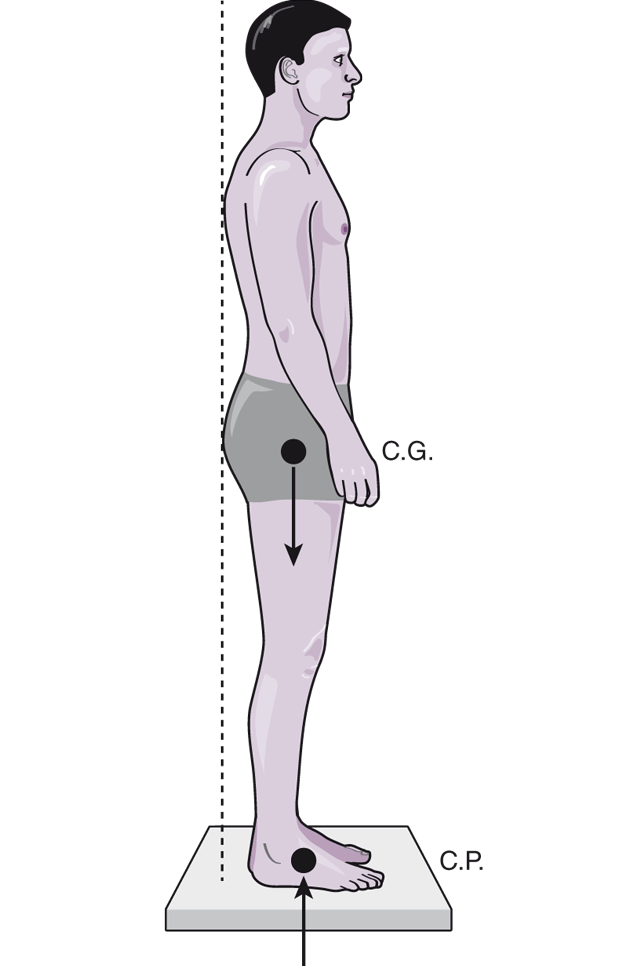
\includegraphics[height=0.3\textwidth]{Posture-et-equilibre1.png}
        \end{figure}
    \end{center}
    \begin{center}
        \begin{tabular}{lll}
            
            \Large {Résponsable d'UE} & \Large Gilles Lepinard & \Large gilles.lebinard@laposte.fr
        \end{tabular}
    \end{center}
    \begin{center}
        \emph{2022/2023}
    \end{center}

    \newpage
        \tableofcontents
    \newpage
        \section{Introduction}
        Le KOM s'est tenu le 10/01/2023 à l'IRIT, réunissant les participants suivants : 

            - Bilel Besseghieur "Chef de projet -équipe-".

            - Khalil Maachou "Developpeur -équipe-".

            - Mamadou Djibo Soungouli "Developpeur -équipe-".

            - Sandrine Mouysset "Cliente".

            - Clément Regis "AMO".

        L'objectif de cette réunion était de lancer le projet en discutant les détails du plan d'action, les tâches à accomplir et les délais pour chaque étape de ce projet.

        Au cours de cette réunion, les différentes responsabilités et les rôles de chaque membre de l'équipe ont été définis, ainsi que les objectifs à atteindre pour le projet.
        Des décisions importantes ont également été prises en ce qui concerne les ressources nécessaires, les échéanciers et les mécanismes de suivi pour assurer le bon déroulement du projet.

        Il a également été discuté des éventuels obstacles et des risques potentiels que pourrait rencontrer le projet et des mesures pour les gérer. Enfin, les prochaines étapes ont été planifiées pour assurer la mise en place efficace de toutes les actions décidées lors de cette réunion KOM.

        \section{Observation}

            \subsection{Fonctionnement}
            Lors de la discussion avec le client concernant le fonctionnement le client ne souhaite pas le changer sauf:  

            - il ne souhaite pas nécessairement avoir accès au github du projet.

            - la partie classification et design final dans notre diagram de GANT c'est pas 

                critique sauf si on a le temps et les moyens (Les donneées de tests) dans le livrable 

                final c'est une application mobile qui récupere les données de posturales.
                
            \subsection{Rôles}
                Les rôles attribués et les activitées préciser pour chaque membre de groupe convient au client donc y aura aucune modification.

            \subsection{Technologie}
                Puisque l'objectif à été modifié, Le client a prciser que sert a rien pour le moment parce qua la partie classification est facultatif pour l'instant.

            \subsection{Objectif}

                L'objectif que le client à en tête est légèrement différent, il souhaite d'abord une application qui puisse récupérer les données des capteurs gyroscopiques, les stocker et les exploiter pour le sujet (analyse des mesures posturales d'une personne).

                Éventuellement une fois cela fait, pouvoir faire une prédiction, mais cela est facultatif (si cela est réalisable).
            
            \section{Les actions et décisions}

            \subsection{Fonctionnement}

            \subsection{Technologie}
                python ne sera peut-être pas utilisé pour ce projet, l'utilisation de Kotlin pour l'application android convient au client.
            
        \section{Conclusion}
            Ce kick-off meeting nous à permis de clarifier le projet avec le client, notamment sur l'objectif et de mieux comprendre la ligne à suivre. Cela à permis aussi de clarifier le rôle de Clément Régis au sein de notre équipe.
\end{document}